%% Beamer Presentation using 16:9 aspect ratio (HDTV standard aspect ratio)
\documentclass[aspectratio=169]{beamer}

%% Metropolis or mtheme Theme
\usetheme{metropolis}

% Packages
\usepackage{fancyvrb}
\usepackage{graphicx}
\usepackage{listings}
\usepackage[]{hyperref, amsmath}
\usepackage{pgfplots}
\usepackage{appendixnumberbeamer}
\usepackage{enumitem}
\usepackage[caption=false]{subfig}
\usepgfplotslibrary{statistics}
%\usepgfplotslibrary{external} 
%\tikzexternalize

% Provide an easy command for mono spaced font: \t{text}
\renewcommand{\t}[1]{\texttt{#1}}

% Provide an easy command for full screen graphics
\newcommand<>{\fullsizegraphic}[1]{
{
    \begin{frame}[plain]
        \begin{tikzpicture}[remember picture,overlay]
            \node[at=(current page.center)] {
                \includegraphics[width=\paperwidth]{#1}
            };
        \end{tikzpicture}
    \end{frame}
}
}
\newcommand<>{\fullsizegraphich}[1]{
{
    \begin{frame}[plain]
        \begin{tikzpicture}[remember picture,overlay]
            \node[at=(current page.center)] {
                \includegraphics[height=\paperheight]{#1}
            };
        \end{tikzpicture}
    \end{frame}
}
}

% Customize the Fancy Verbatim environment's default font and margins
\RecustomVerbatimEnvironment
{Verbatim}{Verbatim}
{formatcom=\scriptsize,xleftmargin=0.75ex}

% use filled blocks for default, alert and example blocks
\metroset{block=fill}

% Title format uses smallcaps
\metroset{titleformat=smallcaps}

% 42 Lines logo colors
\definecolor{blue}{RGB}{5,76,111}
\definecolor{lightblue}{RGB}{53,137,175}
\definecolor{grey}{RGB}{187,187,187}

% Adjust Metropolis theme to use 42 Lines colors
\setbeamercolor{alerted text}{fg=lightblue}
\setbeamercolor{example text}{fg=blue}
\setbeamercolor{palette primary}{bg=blue}

% Customization for code listings including font size, a background and margins
\lstset{
    basicstyle=\tiny\ttfamily,
    backgroundcolor=\color{normal text.bg!80!normal text.fg!50!normal text.bg},
    frame=single,
    framerule=0pt,
}

% Here ends the preamble


\title{Observability Data Engineering}
\subtitle{A Story About Math, Four Golden Signals, and Business Intelligence}
\institute{DevOps Observability Architect}
\author{Jack Neely\\ jjneely@gmail.com}

\date{\today}

\newcommand{\hcancel}[1]{%
    \tikz[baseline=(tocancel.base)]{%
        \node[inner sep=0pt,outer sep=0pt] (tocancel) {#1};
        \draw[lightblue, very thick] (tocancel.south west) -- (tocancel.north east);
    }%
}%

\begin{document}

%% Introduction, Title
\maketitle

%% In the Before Time Lightning Talk
%% Consultant work
\begin{frame}
    \frametitle{Monitorama PDX 2019: How to know if something is ``up''}
    \begin{tikzpicture}[remember picture,overlay]
        %%\node[at=(current page.center)] {
        %%    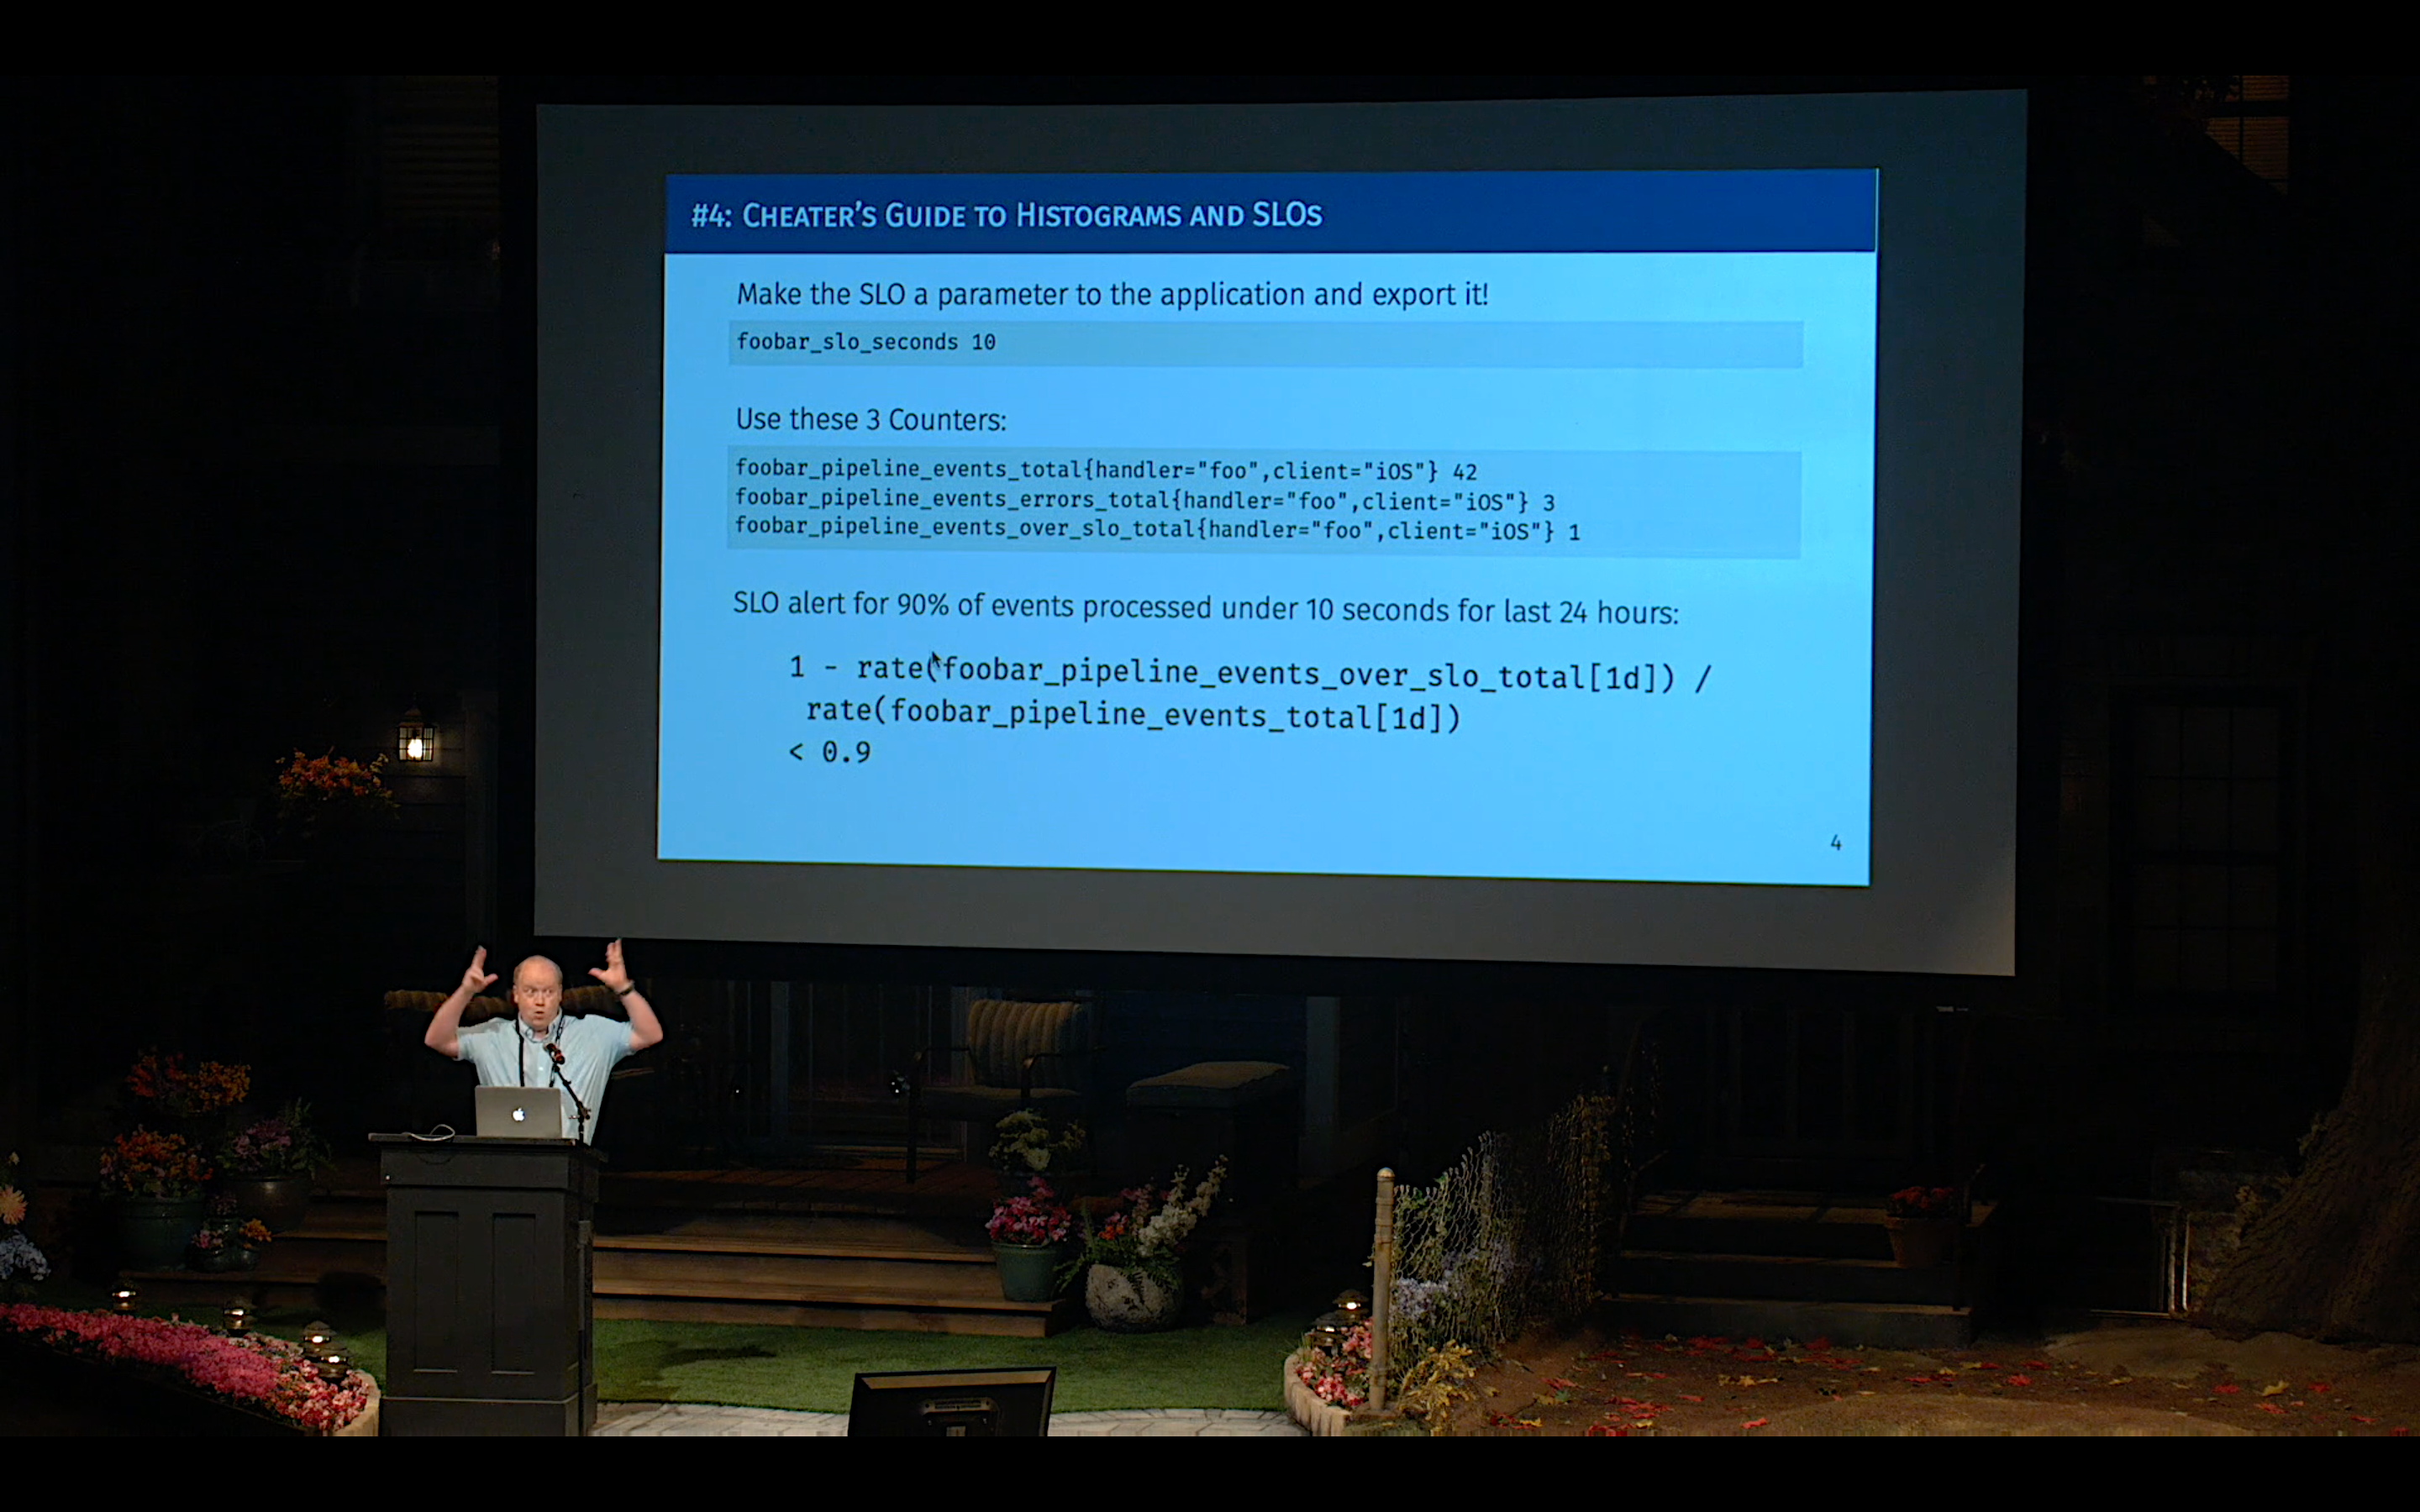
\includegraphics[width=10cm]{img/lightning-2019.png}
        %%};
    \end{tikzpicture}
\end{frame}

\begin{frame}
    \frametitle{As a DevOps Observability Architect...}

    \emph{What do I monitor?}

    Google SRE's \hcancel{Four} Five Golden Signals
    \begin{description}
        \item[Health] Pods are Running and Healthy
        \item[Traffic] Counter of Units of Work
        \item[Errors] Counter of Units of Work with Exceptions
        \item[Latency] Timer of the distribution of latencies for each Unit of Work
        \item[Saturation] When Pods be scaled up or down
    \end{description}

    Remember: \alert{There are FIVE lights!}
\end{frame}

\begin{frame}
    \frametitle{As a DevOps Observability Architect...}

    The \hcancel{Four} Five Golden Signals is knowing before the customers do.

    \pause
    \begin{quote}
        \emph{We need to set alerts for these super special customers.}
    \end{quote}

    Well, if we set our Histograms correctly and record maximum values we will
    be able to tell when...

    \pause
    \begin{quote}
        \emph{When a customer calls we need to be able to verify the error
            they encountered.  We'll need a high cardinally solution.}
    \end{quote}

    Umm...those aren't metrics.  How heavily are you sampling your traces?

    \pause
    \begin{quote}
        \emph{Jack, we're an Enterprise!}
    \end{quote}
\end{frame}

\begin{frame}
    starship goes here
\end{frame}

\frame[standout]{Traffic}

%% Count Units of Work
%% Why Counting monotonoically matters like a network device

\begin{frame}
    \frametitle{Why Counters Work}

    \begin{quote}
         Systems based in cumulative monotonic sums are naturally simpler, in
         terms of the cost of adding reliability. When collection fails
         intermittently, gaps in the data are naturally averaged from
         cumulative measurements.  -- OpenTelemetry Data Model
    \end{quote}

    Most Accurate: Incremented in discrete whole numbers.  Never misses an
    event.

    Synchronization Primitive: Allows for multiple observers.

    Low Overhead: Easy implementation.  No copying or recalling previous
    values.

    Fundamental: \textbf{Position!}

    %% https://www.researchgate.net/publication/3849082_Monotonic_counters_A_new_mechanism_for_thread_synchronization
\end{frame}

\begin{frame}
    \frametitle{Remembering Physics}
    \begin{columns}
        \begin{column}{0.33\textwidth}
            Position
            \resizebox{\columnwidth}{!}{\begin{tikzpicture}[/pgf/declare function={f=3*x^3-6*x^2+2*x-1;}]
\begin{axis}[
    domain=0:10,
    ymax=2500,
    samples=100,
    axis lines=middle,
    xticklabel=$t_{\pgfmathprintnumber{\tick}}$
]
\addplot [thick] {f};
\end{axis}
\end{tikzpicture}
}
        \end{column}
        \begin{column}{0.33\textwidth}
            Velocity
            \resizebox{\columnwidth}{!}{\begin{tikzpicture}[/pgf/declare function={f=9*x^2 - 12*x + 2;}]
\begin{axis}[
    domain=0:10,
    ymax=2500,
    samples=100,
    axis lines=middle,
    xticklabel=$t_{\pgfmathprintnumber{\tick}}$
]
\addplot [thick] {f};
\end{axis}
\end{tikzpicture}
}
        \end{column}
        \begin{column}{0.33\textwidth}
            Acceleration
            \resizebox{\columnwidth}{!}{\begin{tikzpicture}[/pgf/declare function={f=18*x - 12;}]
\begin{axis}[
    domain=0:10,
    ymax=2500,
    samples=100,
    axis lines=middle,
    xticklabel=$t_{\pgfmathprintnumber{\tick}}$
]
\addplot [thick] {f};
\end{axis}
\end{tikzpicture}
}
        \end{column}
    \end{columns}
    \note[item]{Spike detection}
\end{frame}

\begin{frame}[fragile]
    \frametitle{Counting Caveats: Riemann Sums}
    \note[item]{How to aggregate Counters}
    \begin{columns}
        \begin{column}{0.5\textwidth}
            \resizebox{\columnwidth}{!}{\pgfplotsset{
    integral segments/.code={\pgfmathsetmacro\integralsegments{#1}},
    integral segments=10,
    integral/.style args={#1:#2}{
        ybar interval,
        domain=#1+((#2-#1)/\integralsegments)/2:#2+((#2-#1)/\integralsegments)/2,
        samples=\integralsegments+1,
        x filter/.code=\pgfmathparse{\pgfmathresult-((#2-#1)/\integralsegments)/2}
    }
}

%% https://math.dartmouth.edu/opencalc2/cole/lecture8.pdf
%%\begin{tikzpicture}[/pgf/declare function={f=0.1*x^2+1;}]
\begin{tikzpicture}[/pgf/declare function={f=3*x^3-6*x^2+2*x-1;}]
\begin{axis}[
    domain=0:10,
    samples=100,
    axis lines=middle,
    xticklabel=$t_{\pgfmathprintnumber{\tick}}$
]
\addplot [
    red,
    fill=red!50,
    integral=0:10
] {f};
\addplot [thick] {f};
\end{axis}
\end{tikzpicture}
}
        \end{column}
        \begin{column}{0.5\textwidth}
\begin{lstlisting}
interval: 5m
rules:
- record: labels:http_server_requests:rate5m
  expr: >
    sum by (service, namespace, status) (
      rate(http_server_requests_seconds_count{}[5m])
    )
\end{lstlisting}

Integrate and Build Ratio:
            \begin{lstlisting}
1 - (
  sum_over_time(
    sum without (status) (
      labels:http_server_requests:rate5m{
        status=~"5..", service="..."})[7d:5m]
  ) * 300 /
  sum_over_time(
    sum without (status) (
      labels:http_server_requests:rate5m{
        service="..."})[7d:5m]
  ) * 300
)
            \end{lstlisting}
        \end{column}
    \end{columns}
\end{frame}

\frame[standout]{Errors}

%% Count Units of Work that fail or create an exception
%% How you CPU metrics are wrong

\begin{frame}[fragile]
    \frametitle{Measuring CPU Usage Over Time}

    How do you measure CPU usage of a process?
    \begin{enumerate}[label=\alph*.]
        \item Jiffies
        \item Percentages
        \item Seconds a Process is in the Running State
        \item All of the above
    \end{enumerate}
\end{frame}

\begin{frame}
    \frametitle{Nyquist-Shannon Sampling Theorem}

\end{frame}

\frame[standout]{Latency}

%% Latency: Timers and Distributions -- Why averages are horrible and
%% Anscombe's Quartet. Understanding Gamma Distributions.

\frame[standout]{Saturation}

%% Saturation: Percentiles and Pipelines -- Visualizing percentiles of data,
%% why we cannot combine percentiles, and the magic of histograms.

\frame[standout]{Customers}

%% T-Digests

\end{document}
